\section{Confidence Intervals}
\label{sec:confidence-intervals}

When we report an estimator $\hat{\theta}$ of a population parameter $\theta$, we know that most likely
\begin{equation*}
  \hat{\theta} \neq \theta
\end{equation*}
due to a sampling error. We realize that we have estimated $\theta$ up to \textit{some error}.

Then how much can we trust the reported estimator? How far can it be from the actual parameter of interest? What is the probability that it will be reasonably close? And if we observed an estimator $\hat{\theta}$, then what can the actual parameter $\theta$ be?

To answer these questions, statisticians use \textbf{confidence intervals}, which contain parameter values that deserve some confidence, given the observed data.
\begin{definition}{}
  An interval $\left[ a,\ b \right]$ is a $(1 - \alpha)100\%$ \textbf{confidence interval} for the parameter $\theta$ if it contains the parameter with probability $(1 - \alpha)$,
  \begin{equation*}
    \prob{a \leq \theta \leq b} = 1 - \alpha
  \end{equation*}
  The \textbf{coverage probability} $(1 - \alpha)$ is also called a \textbf{confidence level}.
\end{definition}

Let us take a moment to think about this definition. The probability of a random event $\{ a \leq \theta \leq b \}$ has to be $(1 - \alpha)$. What randomness is involved in this event?

The population parameter $\theta$ is not random. It is a \textit{population feature, independent of any random sampling procedure}, and therefore, it remains constant. On the other hand, the interval is computed from random data, and therefore, it is random. The coverage probability refers to the chance that our interval covers a constant parameter $\theta$.

\begin{figure}[H]
  \centering
  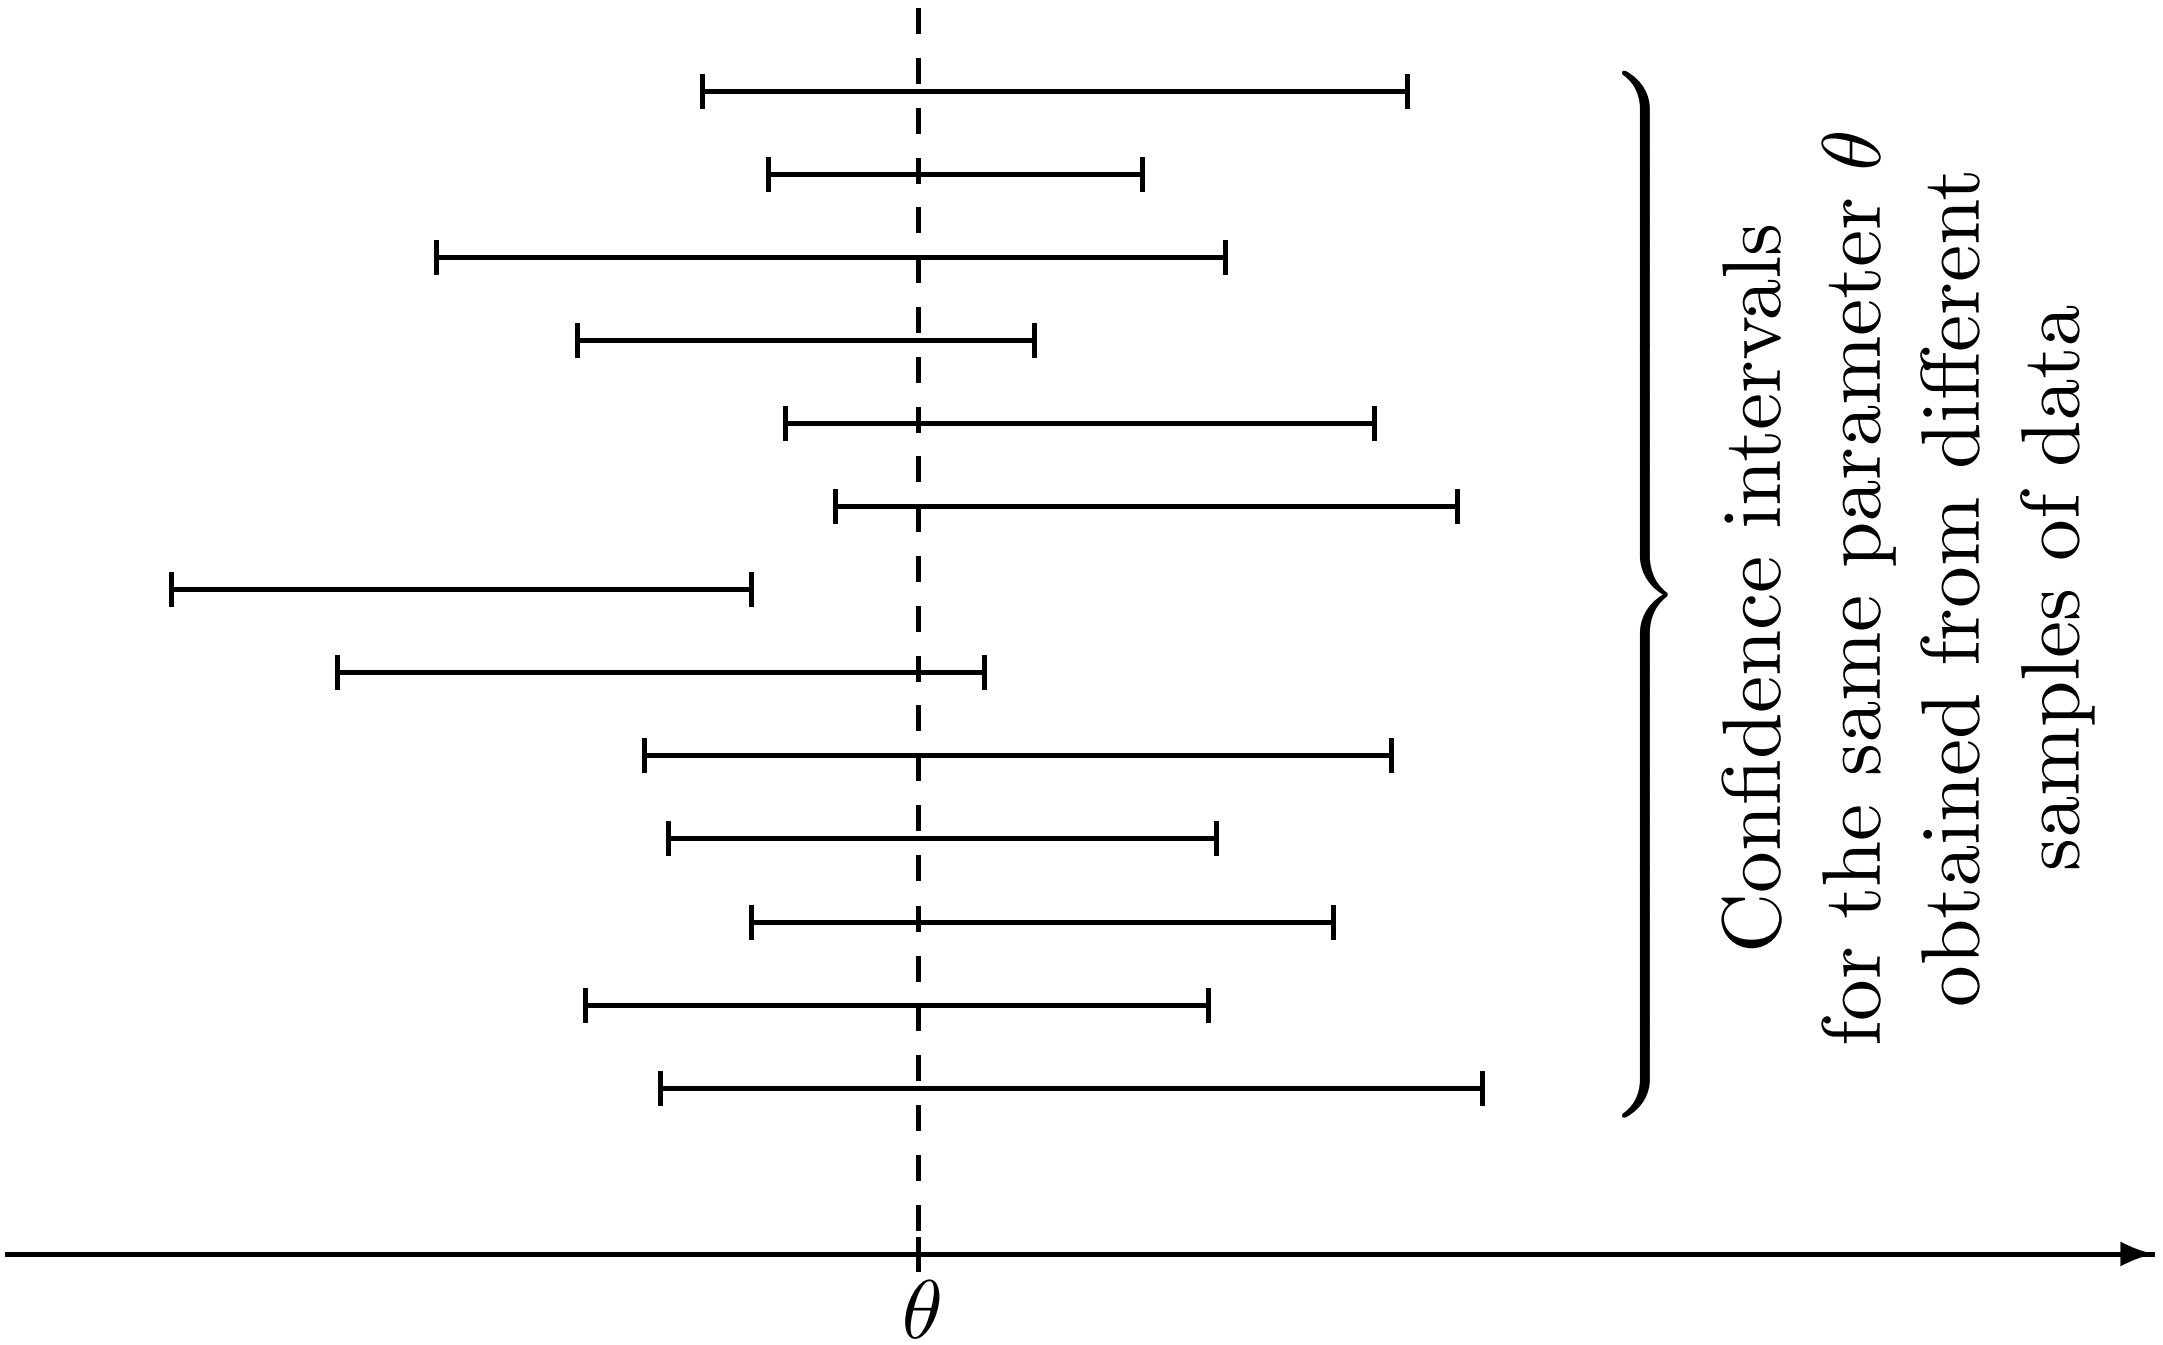
\includegraphics[width=\linewidth]{img/fig-9.2.png}
  \caption{}
  \label{fig:9.2}
\end{figure}

This is illustrated in Figure 2. Suppose that we collect many random samples and produce a confidence interval from each of them. If these are $(1 - \alpha)100\%$ confidence intervals, then we expect $(1 - \alpha)100\%$ of them to cover $\theta$ and $100\alpha\%$ of them to miss it. In Figure 2, we see one interval that does not cover $\theta$. No mistake was made in data collection and construction of this interval. It missed the parameter only due to a \textit{sampling error}.

It is therefore wrong to say, ``I computed a $90\%$ confidence interval, it is $\left[ 3,\ 6 \right]$. Parameter belongs to this interval with probability $90\%$''. The parameter is constant; it either belongs to the interval $\left[ 3,\ 6 \right]$ (with probability $1$) or does not. In this case, $90\%$ refers to the proportion of confidence intervals that contain the unknown parameter in a long run.

\subsection{Construction of Confidence Intervals: A General Method}
\label{subsec:const-of-conf-inter-a-gen-method}

Given a sample of data and a desired confidence level $(1 - \alpha)$, how can we construct a confidence interval $\left[ a,\ b \right]$ that will satisfy the coverage condition
\begin{equation*}
  \prob{a \leq \theta \leq b} = 1 - \alpha
\end{equation*}
in definition 4.

We start by estimating parameter $\theta$. Assume there is an unbiased estimator $\hat{\theta}$ that has a Normal distribution. When we standardize it, we get a Standard Normal variable
\begin{equation*}
  Z = \frac{\hat{\theta} - \mathbf{E}(\hat{\theta})}{\sigma(\hat{\theta})} = \frac{\hat{\theta} - \theta}{\sigma(\hat{\theta})}
\end{equation*}
where $\mathbf{E}(\hat{\theta}) = \theta$ because $\hat{\theta}$ is unbiased, and $\sigma(\hat{\theta}) = \sigma(\hat{\theta})$ is its standard error.

\vspace*{\fill}
\columnbreak

This variable falls between the Standard Normal quantiles $q_{\alpha/2}$ and $q_{1 - \alpha/2}$, denoted by
\begin{align*}
  - z_{\alpha/2} &= q_{\alpha / 2}\\
  z_{\alpha/2} &= q_{1 - \alpha / 2}\\
\end{align*}
with probability $(1 - \alpha)$, see Figure 3.
\begin{figure}[H]
  \centering
  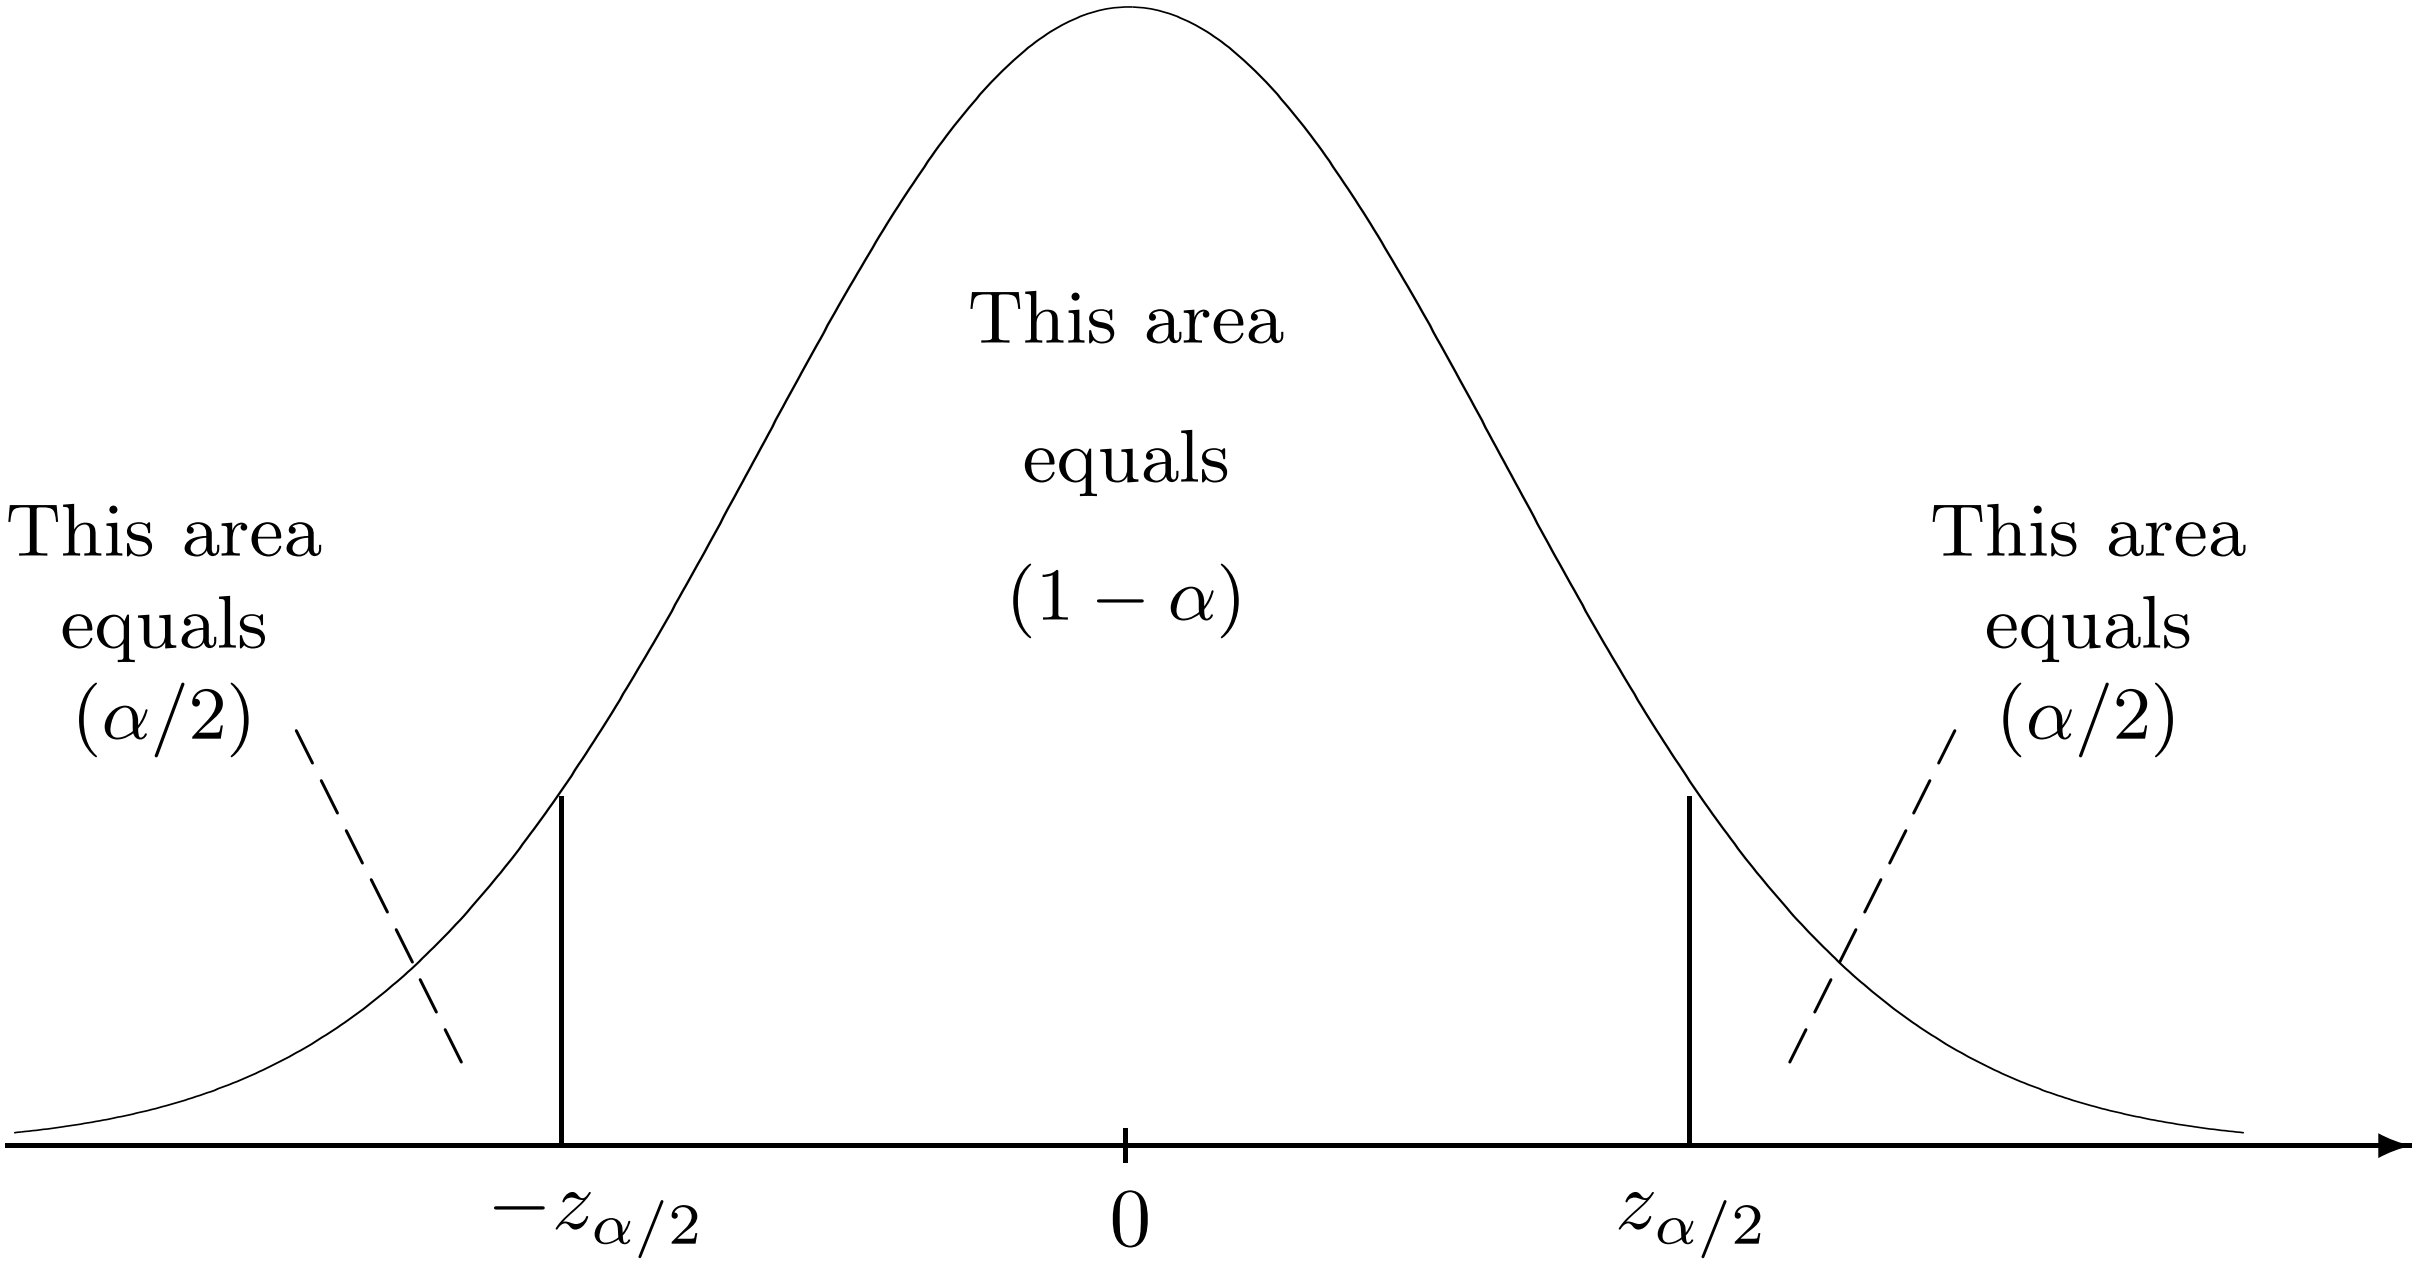
\includegraphics[width=\linewidth]{img/fig-9.3.png}
  \caption{}
  \label{fig:9.3}
\end{figure}

\noindent Then,
\begin{equation*}
  \prob{- z_{\alpha/2} \leq \frac{\hat{\theta} - \theta}{\sigma(\hat{\theta})} \leq z_{\alpha/2}} = 1 - \alpha
\end{equation*}
\noindent Solving the inequality inside $\{ \ldots \}$ for $\theta$, we get
\begin{equation*}
  \prob{
    \hat{\theta} - z_{\alpha/2} \cdot \sigma(\hat{\theta})
    \leq 
    \theta
    \leq
    \hat{\theta} + z_{\alpha/2} \cdot \sigma(\hat{\theta})
  } = 1 - \alpha
\end{equation*}
\noindent The problem is solved! We have obtained two numbers
\begin{align*}
  a &= \hat{\theta} - z_{\alpha/2} \cdot \sigma(\hat{\theta})\\
  b &= \hat{\theta} + z_{\alpha/2} \cdot \sigma(\hat{\theta})
\end{align*}
\noindent such that
\begin{equation*}
  \prob{a \leq \theta \leq b} = 1 - \alpha
\end{equation*}

\begin{formula}{Confidence interval, Normal distribution, Eq. 3}
  If parameter $\theta$ has an unbiased, Normally distributed estimator $\hat{\theta}$, then
  \begin{equation*}
    \hat{\theta} \pm z_{\alpha/2} \cdot \sigma(\hat{\theta}) = \left[ \hat{\theta} - z_{\alpha/2} \cdot \sigma(\hat{\theta}), \hat{\theta} + z_{\alpha/2} \cdot \sigma(\hat{\theta}) \right]
  \end{equation*}
  is a $(1 - \alpha)100\%$ confidence interval for $\theta$.

  If the distribution of $\hat{\theta}$ is \textit{approximately} Normal, we get an approximately $(1 - \alpha)100\%$ confidence interval.
\end{formula}

\setcounter{equation}{4}

In this formula, $\hat{\theta}$ is the \textbf{center of the interval}, and $z_{\alpha/2} \cdot \sigma(\hat{\theta})$ is the \textbf{margin}. The margin of error is often reported along with poll and survey results. In newspapers and press releases, it is usually computed for a $95\%$ confidence interval.

\begin{formula}{NOTATION}
  \begin{equation*}
    z_{\alpha} = q_{1 - \alpha} = \Phi^{-1} (1 - \alpha)
  \end{equation*}
  is the value of a Standard Normal variable $Z$ that is exceeded with probability $\alpha$
\end{formula}

\noindent Several important applications of this general method are discussed below. In each problem, we
\begin{enumerate}
  \item Find an unbiased estimator of $\theta$,
  \item Check if it has a Normal distribution,
  \item Find its standard error $\sigma(\hat{\theta}) = \textnormal{Std}(\hat{\theta})$,
  \item Obtain quantiles $\pm z_{\alpha/2}$ from the table of Normal distribution (Table A4 in the Appendix in textbook), and finally,
  \item Apply the rule (3).
\end{enumerate}

\subsection{Confidence Interval for the Population Mean}
\label{subsec:conf-inter-for-the-pop-mean}

Let us construct a confidence interval for the population mean
\begin{equation*}
  \theta = \mu = \expc{X}
\end{equation*}
\noindent Start with an estimator
\begin{equation*}
  \hat{\theta} = \bar{X} = \frac{1}{n} \sum_{i=1}^{n} X_i
\end{equation*}
\noindent The rule (3) is applicable in two cases.
\begin{enumerate}
  \item If a sample $\bs{X} = (X_1,\ \ldots,\ X_n)$ comes from Normal distribution, then $\hat{X}$ is also Normal, and rule (3) can be applied.
  \item If a sample comes from any distribution, but the sample size $n$ is large, then  $\hat{X}$ has an approximately Normal distribution according to the Central Limit Theorem. Then rule (3) gives an approximately $(1 - \alpha)100\%$ confidence interval.  
\end{enumerate}

The followings can be derived
\begin{align*}
  \expc{X} &= \mu &(\textnormal{unbiased estimator})\\
  \sigma(\bar{X}) &= \sigma / \sqrt{n}
\end{align*}
\noindent Then, (3) reduces to the following $(1 - \alpha)100\%$ confidence interval for $\mu$
\begin{formula}{Confidence interval for the mean; $\sigma$ is known}
  \begin{equation}
    \bar{X} \pm z_{\alpha / 2} \frac{\sigma}{\sqrt{n}}
  \end{equation}
\end{formula}
\begin{example}{}
  Construct a $95\%$ confidence interval for the population mean based on a sample of measurements
  \begin{center}
    2.5, 7.4, 8.0, 4.5, 7.4, 9.2
  \end{center}
  if measurement errors have Normal distribution, and the measurement device guarantees a standard deviation of $\sigma = 2.2$. \\

  \textbf{Solution:}
  This sample has size $n = 6$ and sample mean $\bar{X} = 6.50$. To attain a confidence level of 
  \begin{equation*}
    1 - \alpha = 0.95
  \end{equation*}
  we need $\alpha = 0.05$ and $\alpha/2 = 0.025$. Hence, we are looking for quantiles
  \begin{align*}
    q_{0.025} = - z_{0.025} &&\textnormal{and}&& q_{0.975} = z_{0.025}
  \end{align*}
  From Table 4 in textbook, we find that $q_{0.975} = 1.960$. Substituting these values into (9.5), we obtain a $95\%$ confidence interval for $\mu$,
  \begin{align*}
    \bar{X} \pm z_{\alpha / 2} \frac{\sigma}{\sqrt{n}} &= 6.50 \pm 1.960\frac{2.2}{\sqrt{6}}\\
    &= 6.50 \pm 1.76 \textnormal{ or } \left[ 4.74,\ 8.26 \right]
  \end{align*}
\end{example}


\subsection{Confidence Interval for the Difference Between Two Means}
\label{subsec:conf-inter-for-diff-two-means}

Under the same conditions as in the previous section,
\begin{itemize}
  \item Normal distribution of data or
  \item Sufficiently large sample size,
\end{itemize}
\noindent we can construct a confidence interval for the difference between two means.

\begin{figure}[H]
  \centering
  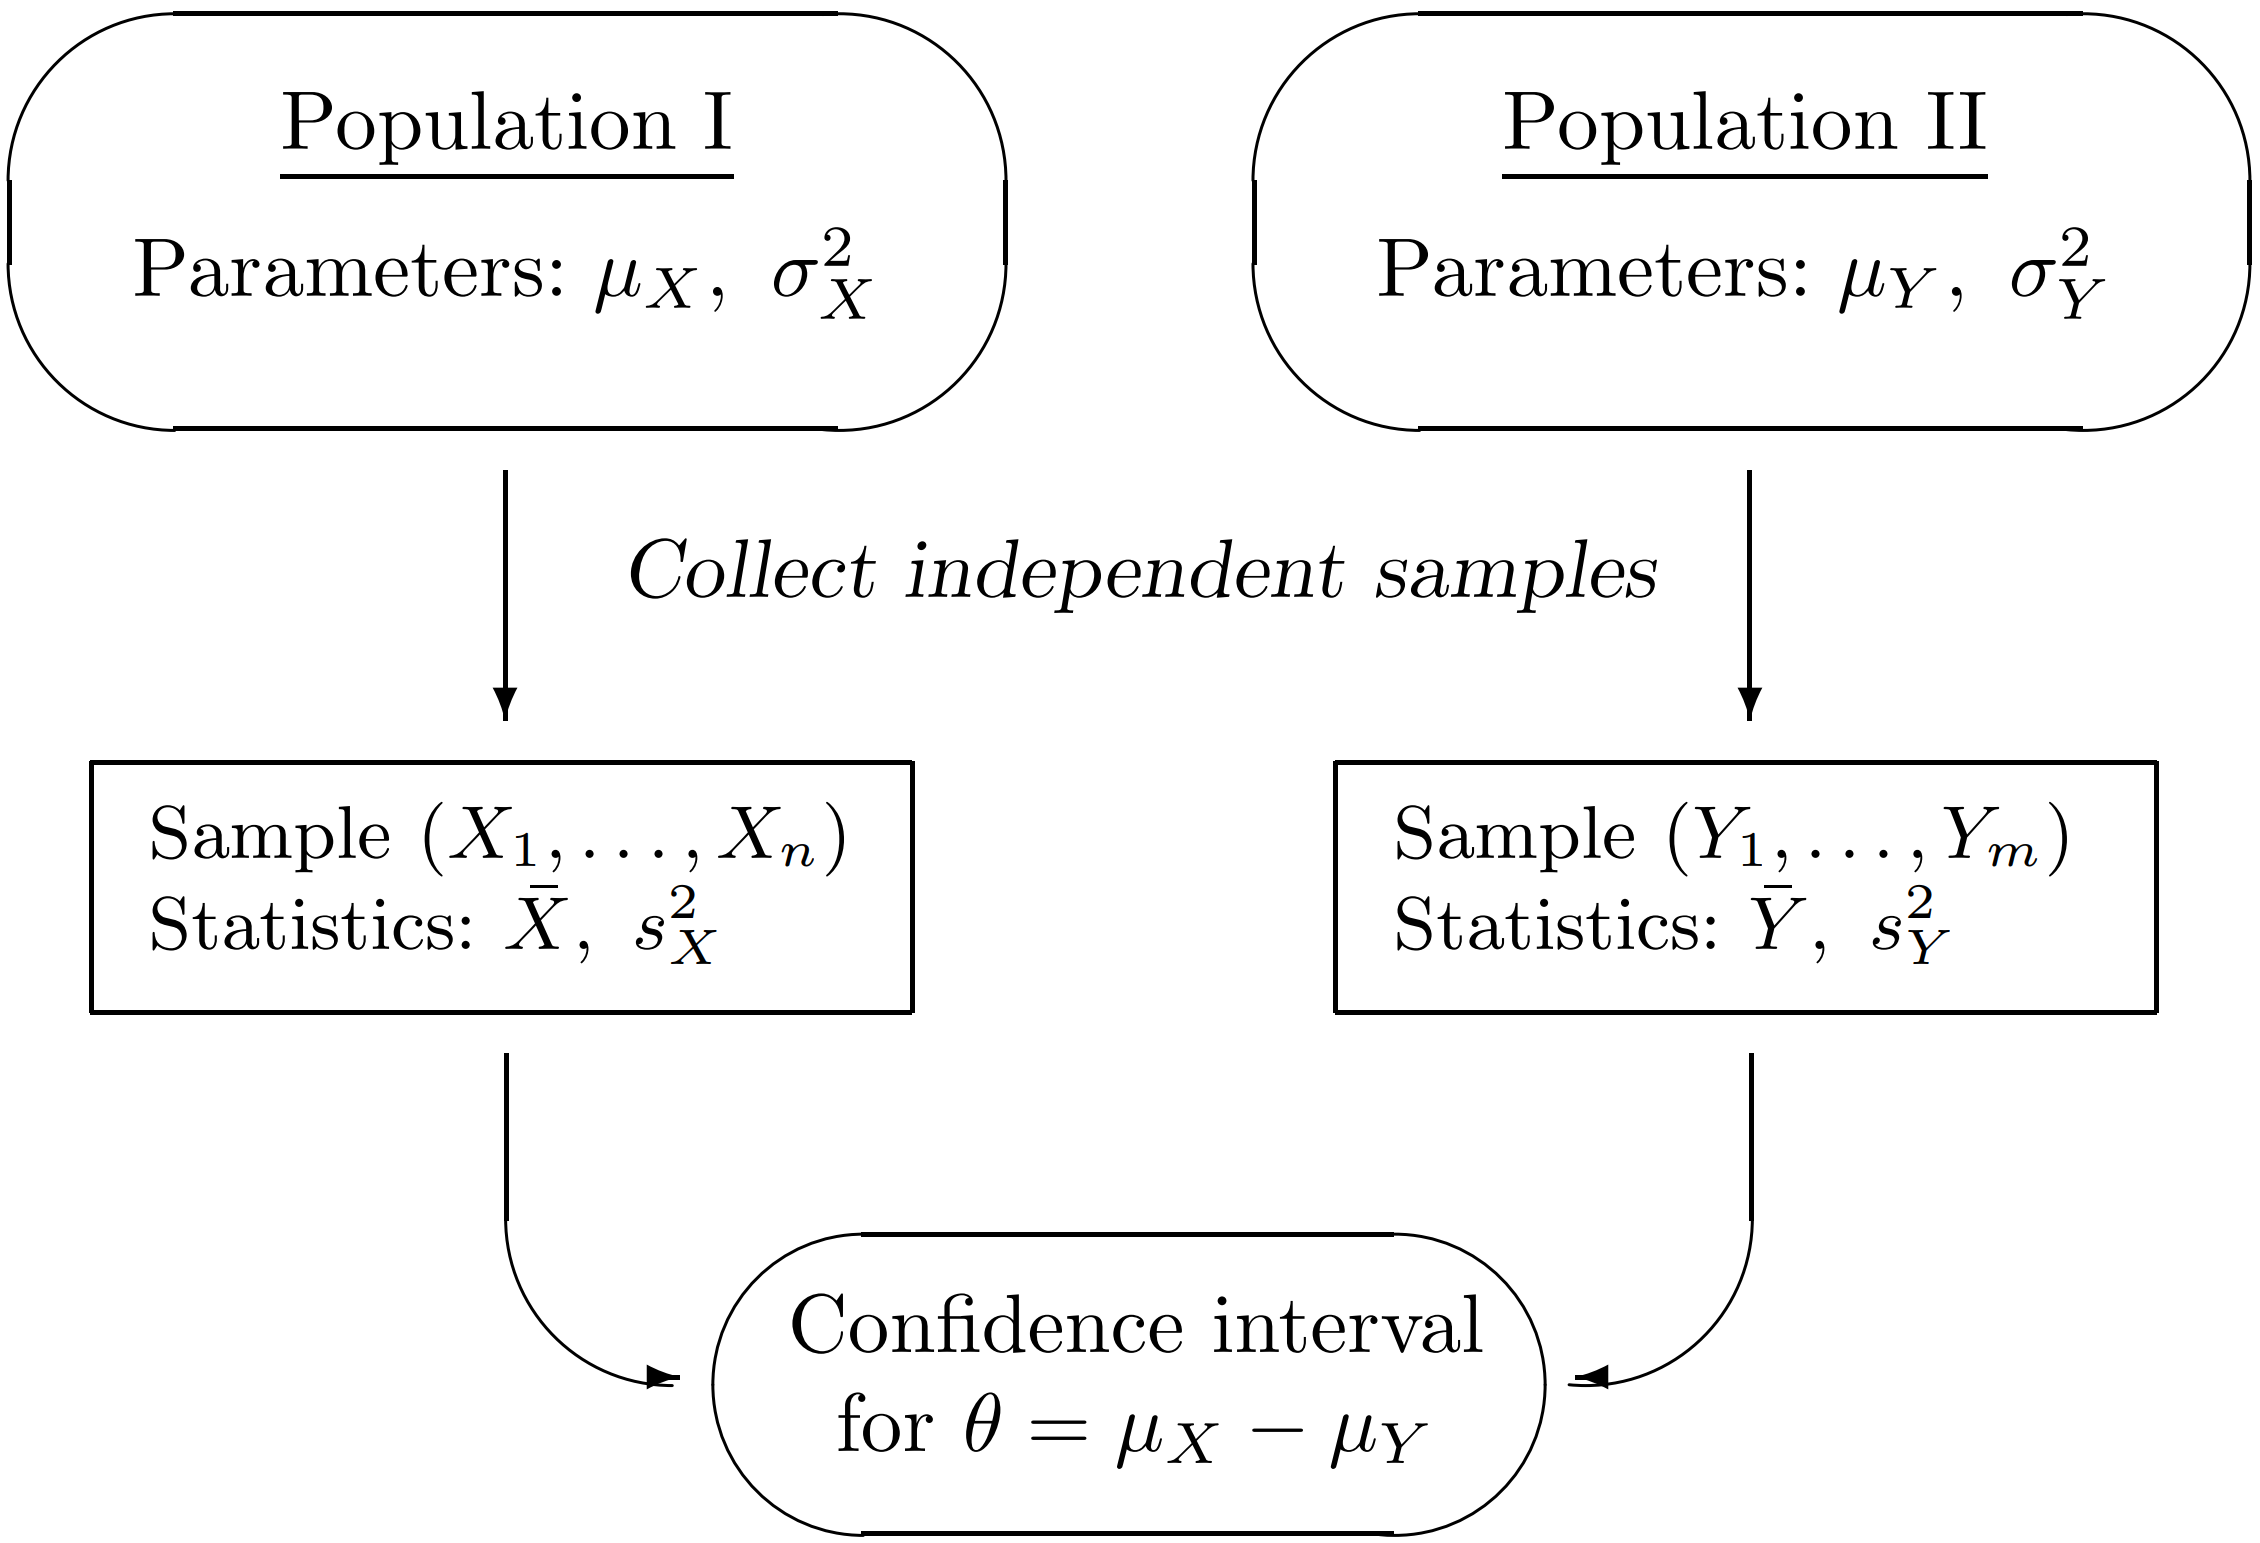
\includegraphics[width=\linewidth]{img/fig-9.4.png}
  \caption{\textit{Comparison of two populations}}
  \label{fig:9.4}
\end{figure}

Suppose that the two samples are collected \textit{independently} of each other. To construct a confidence interval for the difference between population means
\begin{equation*}
  \theta = \mu_X - \mu_Y
\end{equation*}
\noindent we complete the usual steps (a)-(e) below:
\begin{enumerate}[label=(\alph*)]
  \item Propose an estimator of $\theta$,
    \begin{equation*}
      \hat{\theta} = \bar{X} - \bar{Y}
    \end{equation*}
    It is natural to come up with this estimator because $\bar{X}$ estimates $\mu_X$ and $\bar{Y}$ estimates $\mu_Y$.
    \item Check that $\hat{\theta}$ is unbiased. Indeed,
      \begin{equation*}
        \expc{\hat{\theta}} = \expc{\bar{X} - \bar{Y}} = \expc{\bar{X}} - \expc{\bar{Y}} = \mu_X - \mu_Y = \theta
      \end{equation*}
    \item Check that $\hat{\theta}$ has a Normal or approximately Normal distribution. This is true if the observations are Normal or both sample sizes $m$ and $n$ are large.
    \item Find the standard error of $\hat{\theta}$ (using independence of $\bs{X}$ and $\bs{Y}$),
      \begin{align*}
        \sigma(\hat{\theta}) &= \sqrt{\var{\bar{X}} - \var{\bar{Y}}} = \sqrt{\var{\bar{X}} + \var{\bar{Y}}}\\
        &= \sqrt{\frac{\sigma^2_X}{n} + \frac{\sigma^2_Y}{m}}
      \end{align*}
    \item Find quantiles $\pm z_{\alpha/2}$ and compute the confidence interval according to (3). This results in the following formula.
\end{enumerate}
\begin{formula}{Confidence interval for the difference of means; known standard deviations}
  \begin{equation}
    \bar{X} - \bar{Y} \pm z_{\alpha / 2} \sqrt{\frac{\sigma^2_X}{n} + \frac{\sigma^2_Y}{m}}
  \end{equation}
\end{formula}

\begin{example}{ (Effect of an upgrade)}
  A manager evaluates effectiveness of a major hardware upgrade by running a certain process 50 times before the upgrade and 50 times after it. Based on these data, the average running time is 8.5 minutes before the upgrade, 7.2 minutes after it. Historically, the standard deviation has been 1.8 minutes, and presumably it has not changed. Construct a $90\%$ confidence interval showing how much the mean running time reduced due to the hardware upgrade.

  \textbf{Solution:}
  We have $n = m = 50$, $\sigma_X = \sigma_Y = 1.8$, $\bar{X} = 8.5$, and $\bar{Y} = 7.2$. Also, the confidence level $(1 - \alpha)$ equals 0.9, hence $\alpha / 2 = 0.05$, and $z_{\alpha/2} = 1.645$.

  The distribution of times may not be Normal; however, due to large sample sizes, the estimator 
  \begin{equation*}
    \hat{\theta} = \bar{X} - \bar{Y}
  \end{equation*}
  is approximately Normal by the Central Limit Theorem. Thus, formula (6) is applicable, and a $90\%$ confidence interval for the difference of means $(\mu_X - \mu_Y)$ is
  \begin{align*}
    8.5 - 7.2 \pm &1.645 \sqrt{(1.8)^2 \left(\frac{1}{50} + \frac{1}{50}\right)}\\
    &= 1.3 \pm 0.6 \textnormal{ or } \left[ 0.7, 1.9 \right]
  \end{align*}
  We can say that the hardware upgrade resulted in a 1.3-minute reduction of the mean running time, with a $90\%$ confidence margin of 0.6 minutes.
\end{example}

\newpage


\subsection{Selection of a Sample Size}
\label{subsec:selection-of-a-sample-size}

Formula (3) describes a confidence interval as
\begin{center}
  center $\pm$ margin
\end{center}
\noindent where
\begin{align*}
  \textnormal{center} &= \hat{\theta}\\
  \textnormal{margin} &= z_{\alpha / 2} \cdot \sigma(\hat{\theta})
\end{align*}

We can revert the problem and ask a very practical question: \textit{How large a sample should be collected to provide a certain desired precision of our estimator}?

To answer this question, we only need to solve the inequality
\begin{equation}
  \textnormal{margin} \leq \Delta
\end{equation}
in terms of $n$. Typically, parameters are estimated more accurately based on larger samples,
so that the standard error $\sigma(\hat{\theta})$ and the margin are decreasing functions of sample size $n$. Then, (7) must be satisfied for sufficiently large $n$.


\subsection{Estimating Means with a Given Precision}
\label{subsec:estimating-means-with-given-precision}

When we estimate a population mean, the margin of error is
\begin{equation*}
  \textnormal{margin} = z_{\alpha / 2} \cdot \sigma / \sqrt{n}
\end{equation*}
Solving inequality (7) for $n$ results in the following rule.
\begin{formula}{Sample size for a given precision}
  In order to attain a margin of error $\Delta$ for estimating a population mean with a confidence level $(1 - \alpha)$, a simple of size
  \begin{equation}
    n \geq \left( \frac{z_{\alpha/2} \cdot \sigma}{\Delta} \right)^2
  \end{equation}
  is required.
\end{formula}
When we compute the expression in (8), it will most likely be a fraction. Notice that we can only round it up to the nearest integer sample size. If we round it down, our margin will exceed $\Delta$.

Looking at (8), we see that a large sample will be necessary
\begin{itemize}
  \item to attain a narrow margin (small $\Delta$);
  \item to attain a high confidence level (small $\alpha$); and
  \item to control the margin under high variability of data (large $\sigma$).
\end{itemize}
In particular, we need to quadruple the sample size in order to half the margin of the interval.

\begin{example}{}
  In Example 4,  we constructed a $95\%$ confidence with the center $6.50$ and margin $1.76$ based on a sample of size $6$. Now, that was too wide, right? How large a sample do we need to estimate the population mean with a margin of at most $0.4$ units with $95\%$ confidence?

  \textbf{Solution:}
  We have $\Delta = 0.4$, $\alpha = 0.05$, and $\sigma = 2.2$ (from Example 4). By (8), we need a sample of
  \begin{equation*}
    n \geq \left( \frac{z_{0.05 / 2} \sigma}{\Delta} \right)^2 = \left( \frac{(1.960) (2.2)}{0.4} \right)^2 = 116.2
  \end{equation*}
  Keeping in mind that this is the minimum sample size that satisfies $\Delta$, and we are only allowed to round it up, we need a sample of at least 117 observations.  
\end{example}

